%!TEX root=paper.tex

\newpage
\section{What is the Perception of the Learners?}

\subsection{In App Feedback Request}
Besides the analysis that we did based on the observed user data, we also asked the students a series of questions by popping up questions while they are using the sytem (by using an online tool called HotJar). Among the questions was whether they preferred the reading platform and why. Some of the qnswers can be seen in the screenshot below. It becomes clear that the students appreciate the possibility of reading what is interesting for them.

    \begin{figure}[h!]
    \centering
      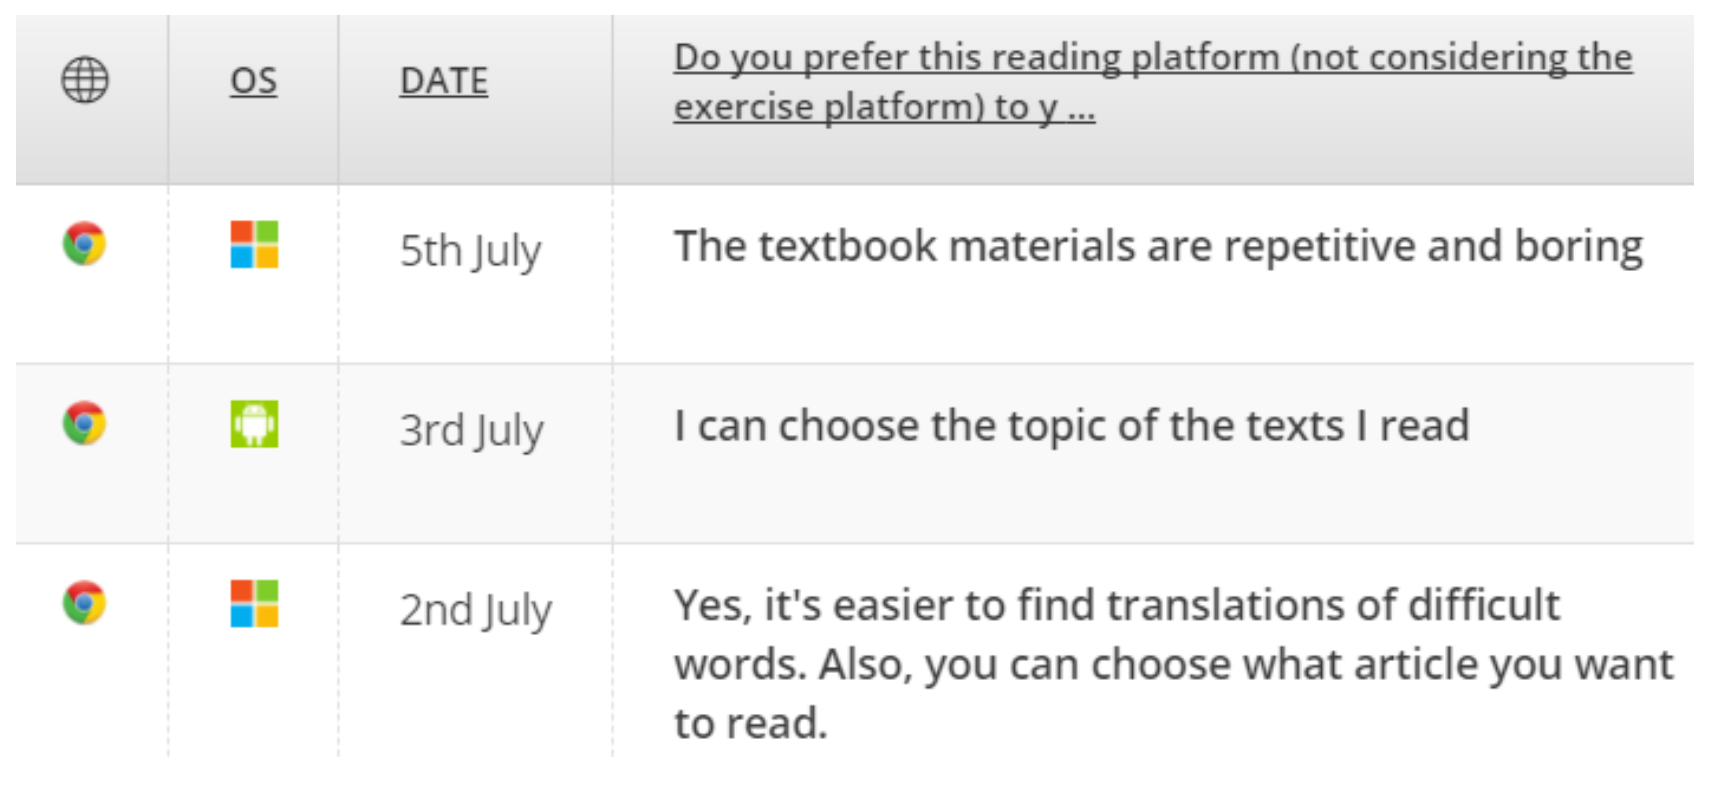
\includegraphics[width=0.9\columnwidth]{figures/opinion_on_reading_platform}
      \caption{The students appreciate the freedom of reading what is interesting to them }
    \end{figure}

\subsection{Post-Usage Survey}

The majority of the students who answered our post-usage survey said that  they prefer our system to a textbook. However, we still think this is not very conclusive since the number of students who answered our survey was quite limited: 12 of the 60 students represent about 20\% of the participants. 


\subsection{Reports to the Teacher}
However, since they might have been more sincere when reporting to their teacher than directly to us, we report here also what they wrote in a separate evaluation of the tools they use in the class, which the teacher runs always at the end of the school year. Several of the answers are: 

\begin{description}
  \item {\em ``It works well but it were better if the translation would have been in Dutch. It is good that you can choose yourself what to read.''}
  \item {\em ``Good for reading skills. It would have been best if it were in Dutch.''}
  \item {\em ``Your vocabulary is really moving forward, but then you have to do it more often than a few times. Overall a nice website, easy and fun subjects''}
\end{description}

There main message in the feedback is that learners appreciate the freedom of chosing materials to read that are personally interesting for them. The second, implied observation is that they appreciate the translations, but they would want to have them in their native language. 

% The way forward is then, by providing better recommendations if possible, and by providing translations in their native languages.

% In the future we plan to investigate whether the system works well enough with Dutch.
